\section{Nächste Nachbar Vorhersage}
\label{sc:theory_nn}
Das Ziel der \textit{nächsten Nachbar Vorhersage} ist es den funktionalen Zusammenhang $F : X \rightarrow Y$ zu finden, welcher Daten der Menge $X \in \mathbb{R}^n$ auf Elemente aus $Y \in \mathbb{R}^m$ eindeutig abbildet. Hierfür wird angenommen, dass die Funktion $F$ lokal stetig ist. Zudem werden hierfür Daten benötigt, anhand derer der Zusammenhang erlernt werden kann.\\
Zu Beginn werden Paare $(\vec{x},\vec{y}) \in X \times Y$ aus einem \textit{Trainingsdatensatz} gebildet und eine Suchstruktur über die $x$-Werte gebildet. Nun kann diese Struktur genutzt werden, um für ein gegebenes $\vec{x}$ den wahrscheinlichsten Wert $\vec{y}$ zu suchen. Hierfür werden, unter der Annahme der lokalen Stetigkeit, die Datenpunkte $\vec{x}_1, ..., \vec{x}_k$ aus der zuvor angelegten Suchstruktur ausgewählt, welche den geringsten Abstand $d(\vec{x}, \vec{x_i})$ zu $\vec{x}$ besitzen.\\
Diesen $k$ Datenpunkten ist jeweils ein eindeutiger Wert $\vec{y}_i$ zuvor zugeordnet werden. Damit kann nun eine Approximation für den zu $\vec{x}$ gehörigen Wert $\vec{y}$ erstellt werden, indem beispielsweise ein gewichteter Mittelwert der $\vec{y}_i$ genutzt wird. Hierzu kann jedem der $k$ nächsten Nachbarn $(\vec{x}_i, \vec{y}_i)$ ein Gewicht $w_i(\vec{x})$ nach
\begin{align*}
w_i(\vec{x}) = \frac{v_i}{\sum_j v_j}, \text{ mit } v_i = \frac{1}{||\vec{x}_i-\vec{x}||} 
\end{align*}
zugeordnet werden. Diese Definition erfüllt $\sum_i w_i = 1$ und ordnen zudem fernen Nachbarn ein geringeres Gewicht zu. Die dabei auftretende Norm $||\ldots |||$ wird im Folgenden als euklidisch angenommen, sofern keine weiteren Angaben existieren. Somit ergibt sich für die gewichtete Vorhersage
\begin{align}
F(\vec{x}) = \vec{y} = \sum^k_i \vec{y}_i \left( \sum_j \frac{||\vec{x}_i-\vec{x}||}{||\vec{x}_j-\vec{x}||} \right) ^{-1}.
\end{align}

Der Schlüssel in der Bewältigung einer solchen Aufgabe liegt hauptsächlich in der Art und Weise, wie die $k$ nächsten Nachbarn gesucht werden. Hierbei wird im Folgenden der Algorithmus \textsc{k-d-tree} ebenso betrachtet wie ein naiver Ansatz. Bei diesem naiven Ansatz (\textit{brute force}) werden die nächsten Nachbarn aus dem unsortierten Trainingsdatensatz durch pures Ausprobieren aller möglichen Punkte ermittelt.

\subsection{k-d-tree}
Ein \textsc{k-d-tree} ist eine Spezialform eines Binärbaumes, und eine oftmals genutzte Methode um Suchvorgänge in Datenstrukturen durchzuführen. Das zugrundeliegende Prinzip eines solchen Baumen ist, dass wenn der Punkt $P_1$ weit entfernt von $P_2$ liegt, aber $P_3$ nahe an $P_2$ liegt, so folgt daraus, dass $P_1$ und $P_3$ weit voneinander entfernt liegen müssen. Durch eine solche Argumentation muss bei einem solchem Suchvorgang die Distanz zweier Punkte seltener berechnet werden, wodurch Rechenzeit eingespart werden kann.\\
 
Der Suchvorgang besteht aus zwei Phasen. Zuerst wird die Aufbauphase des Baumes durchgeführt, bei der die Trainingsdaten einsortiert und damit ein Suchindex erzeugt wird. Anschließend folgt die Suchphase, bei der der zuvor erstellte Suchindex nach dem nächsten Nachbarn durchsucht wird.\\

In der Aufbauphase wird zuerst eine Dimensionen ausgewählt und der Median der Daten in dieser Dimension bestimmt. Anschließend werden die Datenpunkte anhand dieses Wertes in eine Menge unterteilt die nur größere oder nur kleinere Elemente bezogen auf jene Dimension beinhaltet. Die beiden Mengen bilden die ersten Äste des Baumes. Nun wird dieser Schritt rekursiv auf alle Äste angewendet, und die hierbei zum Vergleich genutzte Dimension iteriert \cite{de2000computational}. Dieses Verfahren wird so lange wiederholt, bis eine bestimmte maximale Anzahl $N_{max}$ an Knotenpunkten pro Ast erreicht wird. Ab dieser unteren Grenze wird das Erstellen des Binärbaumes beendet. Ab dieser Grenze benötigt der Zugriff auf die verschiedenen Elemente und das Aufteilen in neue Äste mehr Zeit, als das Berechnen der Abstände zwischen den verbleibenden $N_{max}$ Knoten und dem Suchpunkt. Eine beispielhafte Darstellung des Verfahrens ist in Abbildung \ref{fig:kdtree} zu finden.

\begin{figure}[h]
    \centering
    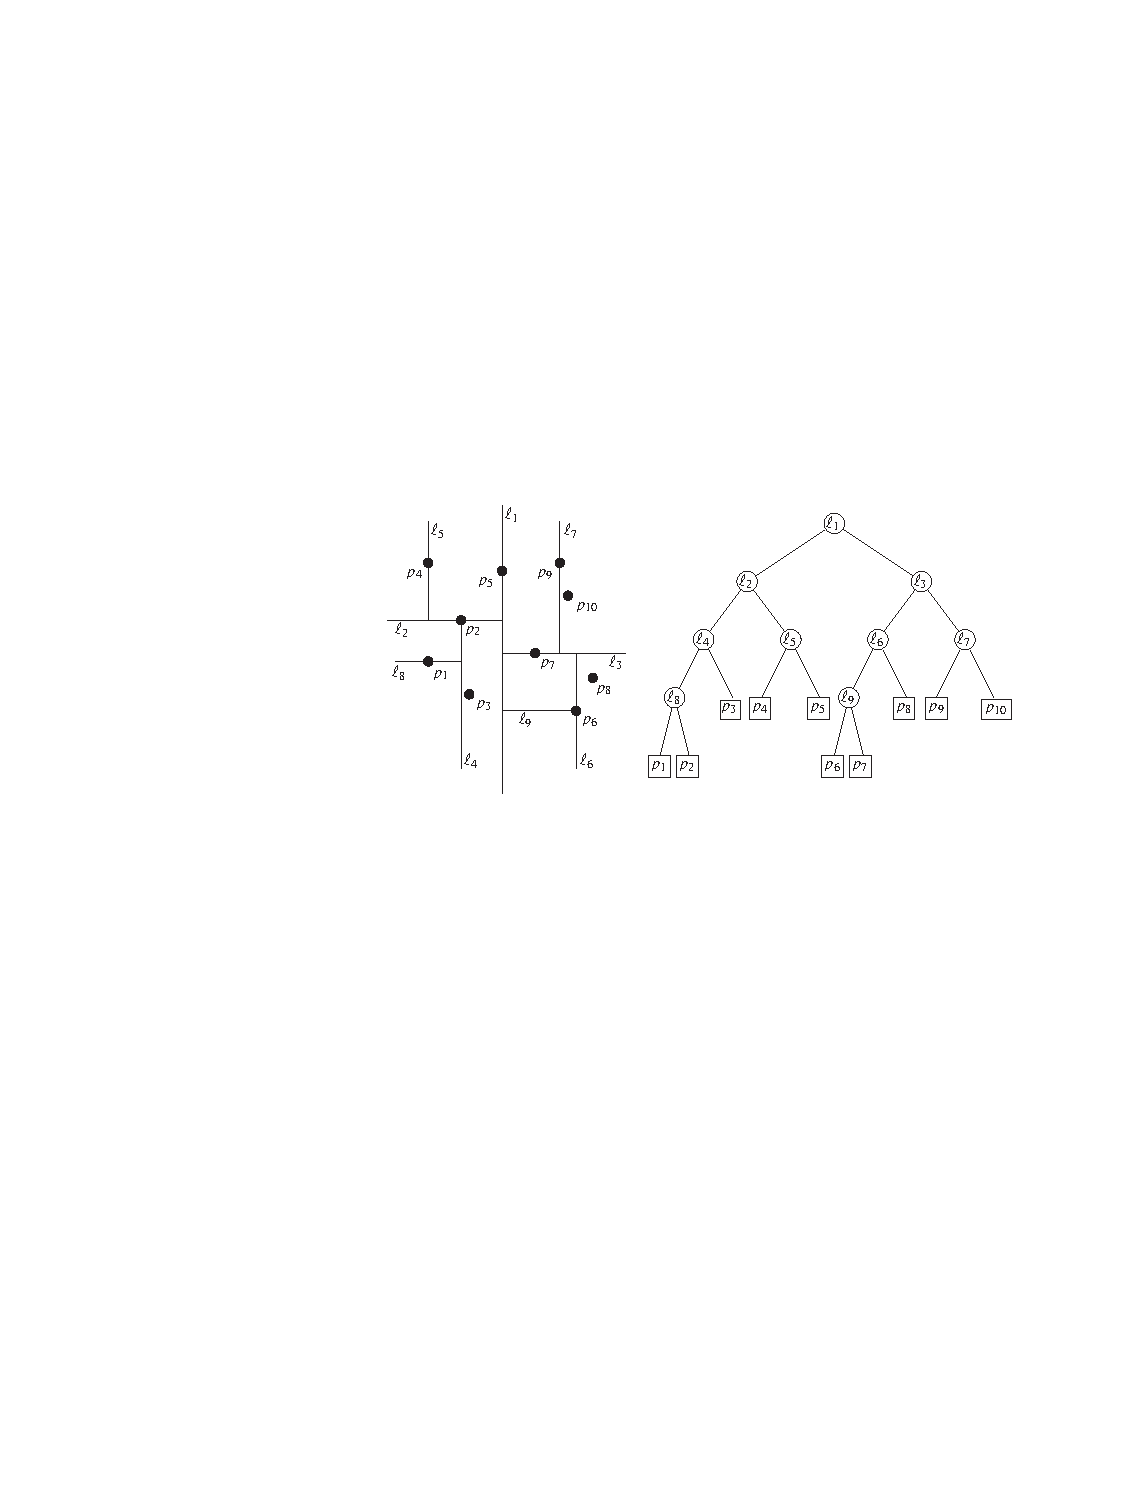
\includegraphics[width = 0.9 \textwidth]{figures/illustrations/kdtree.pdf}
    \caption{Exemplarische Darstellung eines \textsc{k-d-trees} für $d=2$ Dimensionen. In der linkten Hälfte ist die graphische Interpretation der Aufteilung und in der rechten der Aufbau des entstehenden Baumes zu finden \cite{de2000computational}.}
    \label{fig:kdtree}
\end{figure}

Die Suchphase wird nun wieder rekursiv durchgeführt. Hierbei werden wieder iterierend die verschiedenen Dimensionen verglichen, und sich somit immer weiter im Suchbaum nach unten ein Weg gebahnt \cite{de2000computational}. In der untersten Ebene, also wenn nur noch eine Suche zwischen maximal $N_{max}$ Elemente durchgeführt werden muss, wird nun die \textit{brute force}-Suche genutzt. In dieser Arbeit ist für alle Anwendungen diese Schwelle auf $N_{max} = 40$ gesetzt worden.\\

Diese Methode zeichnet sich durch eine Laufzeit, welche sich wie $\mathcal{O}(\log(N))$ verhält, aus \cite{bentley1975multidimensional}. Dies ist geringer, als die Laufzeit eines naiven Suchvorgangs, welche sich wie $N$ verhält. Es hat sich allerdings gezeigt, dass wenn $d$ hinreichend groß ist, diese Vorteile geringer werden, und ab einer gewissen Dimensionalität die Suche langsamer als ein naiver Suchvorgang abläuft.\\

